\newcommand{\drawgraph}{
    \foreach \i in {1,...,9}{
            \pgfmathparse{mod(\i-1,3)} \pgfmathresult %displays 2.0
            \pgfmathtruncatemacro{\x}{\pgfmathresult}  
        
            \pgfmathtruncatemacro{\y}{(\i-1)/3}
        
            \node[draw, circle] (n\i) at (2*\x, 2*\y) {$\i$}; 
        }
        \draw (n1) edge[->] (n5);
        \draw (n2) edge[->] (n4);
        \draw (n5) edge[->] (n3);
        \draw (n5) edge[->] (n6);
        \draw (n6) edge[->] (n9);
        \draw (n6) edge[->] (n8);
        \draw (n5) edge[->] (n8);
        \draw (n3) edge[->] (n6);
        \draw (n4) edge[->] (n5);
       
   }

\newcommand{\drawgraphs}{
    \foreach \i in {1,...,9}{
            \pgfmathparse{mod(\i-1,3)} \pgfmathresult %displays 2.0
            \pgfmathtruncatemacro{\x}{\pgfmathresult}  
        
            \pgfmathtruncatemacro{\y}{(\i-1)/3}
        
            \node[draw, circle] (n\i) at (2*\x, 2*\y) {$\i$}; 
        }
        \draw (n1) edge[red, ultra thick, ->] (n5);
        \draw (n2) edge[red, ultra thick, ->] (n4);
        \draw (n5) edge[red, ultra thick, ->] (n3);
        \draw (n5) edge[->] (n6);
        \draw (n6) edge[red, ultra thick, ->] (n9);
        \draw (n6) edge[red, ultra thick, ->] (n8);
        \draw (n5) edge[->] (n8);
        \draw (n3) edge[red, ultra thick, ->] (n6);
        \draw (n4) edge[->] (n5);
       
   }

\begin{prob}
    Topologically sort the vertices of the following graph. Assume that the nodes are always visited in ascending order, so there is only one correct solution.
    \begin{center}
            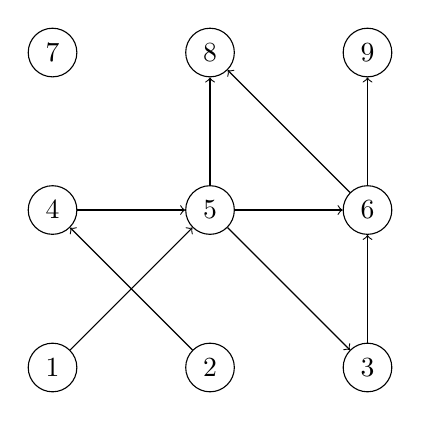
\begin{tikzpicture}
                \drawgraph{}
            \end{tikzpicture}
        \end{center}

    \begin{soln}
    % write your solution here
    \end{soln}
    
    
\end{prob}